\documentclass[aps,prl,preprint,groupedaddress]{revtex4-2}
\usepackage{mhchem, siunitx}
\usepackage[backend=biber]{biblatex}
\addbibresource{references.bib}

\begin{document}
\title{A Rydberg Constant Calculation using the Balmer Series}
\author{Tom Falcone}
\affiliation{Department of Physics, Temple University}
\date{\today}

\begin{abstract}
We used the Rydberg formula with $n_2 = 2$ to estimate the Rydberg constant for hydrogen. The experiment demonstrated that the Bohr model, while obsolete in many regards \cite{krane}, is accurate in its description of state transitions of electrons in the hydrogen atom. Our final calculation of 
$R_H = 1.0975 \pm 0.0010 \times 10^7 ~\si{m^{-1}}$
demonstrates that the Rydberg formula, and consequently its elaboration and explanation given by Bohr, are consistent with experiment.
\end{abstract}

\maketitle

\section{Introduction}
The investigation of various spectral series of hydrogen has led to a better understanding of many phenomena, ranging from atomic structure to the physical properties of astronomical objects. Our experiment is concerned with the visible portion of the Balmer series, discovered by Johann Balmer in 1885\cite{krane}. Not long after his discovery, Johannes Rydberg noticed that the Balmer series along with many other distinct hydrogen spectral series may be described by a general formula,
\begin{align}
    \frac{1}{\lambda}&=R_H~(\frac{1}{n_2^2}-\frac{1}{n_1^2})~.
\end{align}
We'll consider only those wavelengths that are apart of the visible portion of the Balmer series, for which $n_2=2$ is fixed, and $n_1 \in \{2,3,4,5\}$. The aim is to calculate $R_H$ by recording the wavelengths that correspond to intensity peaks in the observed hydrogen spectrum.

\section{Experimental Method}
A hydrogen discharge lamp is set up in front of a digital spectrometer that's hooked up to a computer running Logger Pro software. Electrons are produced at the cathode of the discharge tube and collide with Hydrogen atoms, causing ionization. The ionized hydrogen moves is forced by the electric field toward the cathode, and on its way collides with other hydrogen atoms. In this collision, the electron from the target attaches to the (formerly) ionized hydrogen atom, which cause said atom to emit light at its characteristic wavelengths. This radiation is directed into the digital spectrometer, in which it is diffracted through a grating of known spacing ($d$). Now, the wavelengths of radiation entering the spectrometer can be calculated with $d sin(\phi) = n \lambda$, and the intensity corresponding to radiation at each wavelength is measured. These data are sent to the computer and the spectrum is plotted dynamically as relative intensity vs. wavelength. The position of the lamp relative to the digital spectrometer is adjusted until the highest peak extends precisely the entire height of the graph, at which point we take a snapshot of the spectrum. Finally, a smooth function is constructed from the frozen data by polynomial interpolation. In the regions with wavelengths corresponding to red, blue-green, blue, and violet, the relative maxima are calculated by setting the first order derivative of the interpolation function to 0. The mean intensity peak in each region is calculated with data from 3 trials, and we use equation (1) to estimate $R_H$

\section{Theoretical Background}
The emission of radiation at particular wavelengths by excited hydrogen atoms is explained by Bohr's model of the atom, established in 1913.~\cite{krane} In terms of the Bohr model, $n_1$ and $n_2$ in equation (1) are the initial and final stationary state of an electron that changes energy levels. For hydrogen, the stationary state corresponding to the principle quantum number n has energy 
\begin{align}
    E_n &= -(\frac{e^2}{4 \pi \epsilon_0})^2 \frac{m}{2\hbar^2} \frac{1}{n^2},
\end{align}
and the wavelength of radiation emitted by a transition from state $n_1$ to $n_2$  can be calculated with $E = \frac{hc}{\lambda}$ to get
\begin{align}
    \frac{1}{\lambda}&=(\frac{e^2}{4 \pi \epsilon_0})^{2}\frac{m}{4\pi\hbar^3}(\frac{1}{n_2^2}-\frac{1}{n_1^2})~.
\end{align}
If $m=\frac{m_e m_p}{m_e + m_p}$ (the reduced mass of a hydrogen atom), then $R_H = (\frac{e^2}{4 \pi \epsilon_0})^{2}\frac{m}{4\pi\hbar^3}$. This demonstrates agreement of the various hydrogen spectra with the Bohr model. In fact, the red, blue-green, blue, and violet regions mentioned in the experimental method correspond to an electron changing state from $n_1 = 3, 4, 5,$ or $6$ (respectively) to $n_2 = 2$. By using the wavelength data collected in the experiment and the corresponding value of $n_1$ for each region of the spectrum, we can use equation (1) (with $n_2=2$), to construct a least squares regression line with a slope that estimates $R_H$.

    \begin{figure}[h]
        \centering
		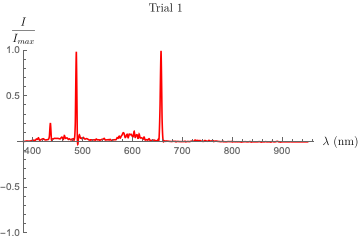
\includegraphics{res/trial1.png}
		\caption{}
    \end{figure}
    
    \begin{figure}[h]
        \centering
		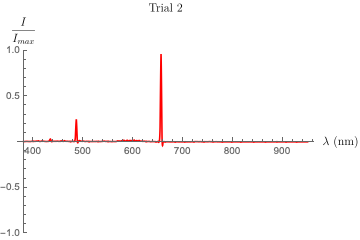
\includegraphics{res/trial2.png}
		\caption{}
    \end{figure}
    
    \begin{figure}[h]
        \centering
		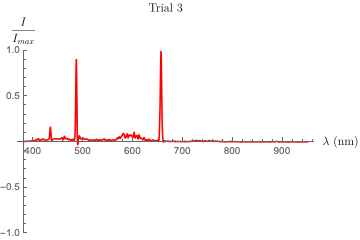
\includegraphics{res/trial3.png}
		\caption{}
    \end{figure}
    
    \begin{table}[h]
        \centering
        \begin{tabular}{||c||c||c||c||} 
             \hline
             $n_1$ & Color & $\lambda_{av}~(\si{nm})$\\ [0.5ex] 
             \hline\hline
             3 & red & 656.0\\ 
             4 & blue-green & 486.0 \\
             5 & blue & 434.0 \\
             6 & violet & 409.9 \\ [1ex] 
             \hline
        \end{tabular}
        \caption{the average wavelength of the intensity peak in each region}
    \end{table}
    
    \begin{figure}[h]
        \centering
		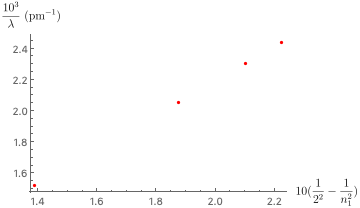
\includegraphics{res/data.png}
		\caption{}
    \end{figure}
\clearpage
\section{Results}
The data in each trial are shown in FIG. 1-3, TABLE I lists the average wavelength of the intensity peaks in each trial, and the discrete measured values that correspond to equation (1) are plotted in FIG 4. Using the method of least squares, we calculated $R_H=1.0975 \pm 0.0001 \times 10^7 ~\si{m^{-1}}$ (an impressive result... had we been attempting to calculate $R_\infty$) This is somewhat consistent with the accepted value, $R_H = 1.09678 \times 10^7 \si{m^{-1}}$, but far from perfect. We now aim to offer an explanation for this slight inaccuracy.
    \begin{figure}
        \centering
        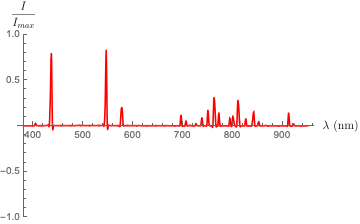
\includegraphics{res/hg.png}
        \caption{}
    \end{figure}
\section{Conclusion}
Of the several pains that could've been taken to increase the accuracy of the experiment, such as a more sensitive spectrometer, or several more trials than just 3, one stands above the rest: the need for isolation of the system from background light. The fluorescent lights in the classroom are mercury discharge lamps. We recorded the spectrum from a (different) mercury discharge lamp and give the results in FIG 5. Since the mercury's radiation has intensity peaks in the same region that we studied with hydrogen radiation, the background radiation from the fluorescent lights skewed the results of the hydrogen spectrum. A simple solution to this problem would be to cover the hydrogen lamp and the spectrometer with an opaque blanket. We estimate the lighting of the environment to give an error in our mean wavelengths of $\Delta \lambda = 1~\si{nm}$. This results in a new calculation of $R_H = 1.0975 \pm 0.0010 \times 10^7~\si{m^{-1}}$, which is indeed more accurate. This final calculation demonstrates a correspondence between the Rydberg formula, the Bohr model, and the true nature of hydrogen emission.

\printbibliography
\end{document}
